\section{Interaction} \label{sec:interaction}
A program called the Scene Generator has been developed to assist in the creation of scenes for SkiROS. Scenes describe the entities that exist in a particular environment in the form of named individuals (i.e. concrete instances) of the classes defined in an ontology. The Scene Generator provides a convenient interface for specifying named individuals of the {\tt paintbot} ontology. The program generates a file in the Turtle format that is ready to be loaded by SkiROS. Figure \ref{fig:scene_generator} shows a sample of the graphical component of the scene generator.

\begin{figure}
    \centering
    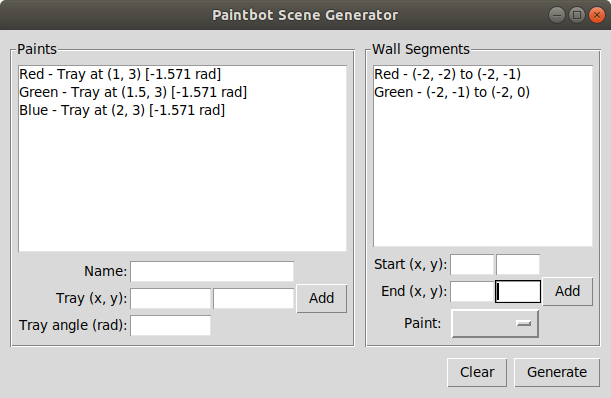
\includegraphics[width=0.75\linewidth]{images/scene_generator.png}
    \caption{The Scene Generator application designed for this project. The left panel allows paints and trays to be specified while the right panel allows wall segments to be specified. This example shows the configuration for one of the scenes used to test the platform.}
    \label{fig:scene_generator}
\end{figure}

The Scene Generator currently supports the specification of paints and walls. When specifying a paint, the user provides its name and both the location and orientation of the tray that contains it. When specifying a wall, the user provides the two endpoints of the wall, $w_0$ and $w_1$, and the color it is to be painted. The line segment defined by the two endpoints is divided into \SI{9}{inch} sections\footnote{\SI{9}{inches} is a very common size for paint rollers.} and the center points of the sections are adjusted so that no section extends past either end of the line segment. This may result in some overlap between sections. The face of the wall that needs to be painted is perpendicular to the line segment and is defined by the following equation:
\[w_\theta = \atantwo(w_{1y} - w_{0y}, w_{1x} - w_{0x}) - \frac{\pi}{2}\]
Any number of paints and walls may be specified using the Scene Generator.

The graphical interface provided by SkiROS is the primary means of interacting with the robot at runtime for this project. More specifically, there are two skills used to perform goal planning and execution: task\_plan and PaintAllWallSections. task\_plan is provided by SkiROS and allows a goal state in PDDL to be specified. This skill sends the goal state to the TFD planner and executes the generated plan. An example goal utilizing the {\tt paintbot} ontology, and the one used in all of the simulations, is {\tt (forall (?w - paintbot:WallSection) (Painted ?w))}. This goal declares that every wall section in the scene must ultimately have the {\tt Painted} property, which is assigned to a wall section upon successful completion of the ApplyPaint skill (see section \ref{sec:task_planning}).

The PaintAllWallSections skill was created in response to observations made during development and testing. This skill causes the robot to paint every wall section in the scene by generating PDDL goals for batches of $10$ sections and invoking the task\_plan skill for each batch. PaintAllWallSections was created to serve two primary purposes: 1) to reduce planning times (see section \ref{sec:results_plan}) and 2) as an exploratory exercise in dynamic planning.

\begin{figure}
    \centering
    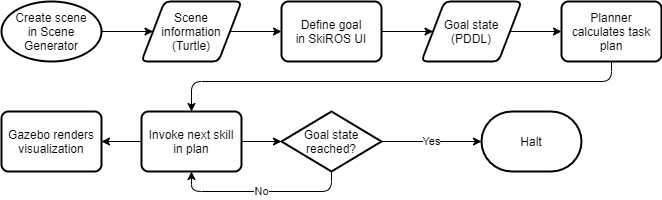
\includegraphics[width=0.75\linewidth]{images/process.png}
    \caption{The general process of using the platform, from generating a scene through the robot executing the tasks to achieve the specified goal.}
    \label{fig:process}
\end{figure}

Figure \ref{fig:process} depicts a high-level overview of the process involved in operating the robot. First, a scene file that represents the entities in the construction environment in the Turtle format needs to be generated. Currently, this needs to be manually done for each new environment the robot will operate in, though work can be done to automate this step. Second, a goal state needs to be provided, as described above. Third, the planner uses the scene information and goal state to calculate the task plan. Finally, the robot executes all skills in the task plan in order.